\documentclass[../main.tex]{subfiles}
 
\begin{document}

Section headings are centered and formatted completely in uppercase 11-point bold font.  Sections should be numbered sequentially, starting with the first section after the Abstract.  The heading starts with the section number, followed by a period.  In LaTeX, a new section is created with the \verb|\section{}| command, which automatically numbers the sections.

Paragraphs that immediately follow a section heading are leading paragraphs and should not be indented, according to standard publishing style\cite{Lamport94}.  The same goes for leading paragraphs of subsections and sub-subsections.  Subsequent paragraphs are standard paragraphs, with 14-pt.\ (5 mm) indentation.  An extra half-line space should be inserted between paragraphs.  In LaTeX, this spacing is specified by the parameter \verb|\parskip|, which is set in {\ttfamily spie.cls}.  Indentation of the first line of a paragraph may be avoided by starting it with \verb|\noindent|.

\subsection{ Main Decoding Processes }

The subsection heading is left justified and set in 11-point, bold font.  Capitalization rules are the same as those for book titles.  The first word of a subsection heading is capitalized.  The remaining words are also capitalized, except for minor words with fewer than four letters, such as articles (a, an, and the), short prepositions (of, at, by, for, in, etc.), and short conjunctions (and, or, as, but, etc.).  Subsection numbers consist of the section number, followed by a period, and the subsection number within that section.  

\subsection{Prediction overview}
The sub-subsection heading is left justified and its font is 10 point, bold.  Capitalize as for sentences.  The first word of a sub-subsection heading is capitalized.  The rest of the heading is not capitalized, except for acronyms and proper names.  

\subsubsection{ Macroblocks and Further Block Division }

\subsubsection{ Intra-Prediction }


   \begin{figure} [ht]
   \begin{center}
   \begin{tabular}{c} %% tabular useful for creating an array of images 
   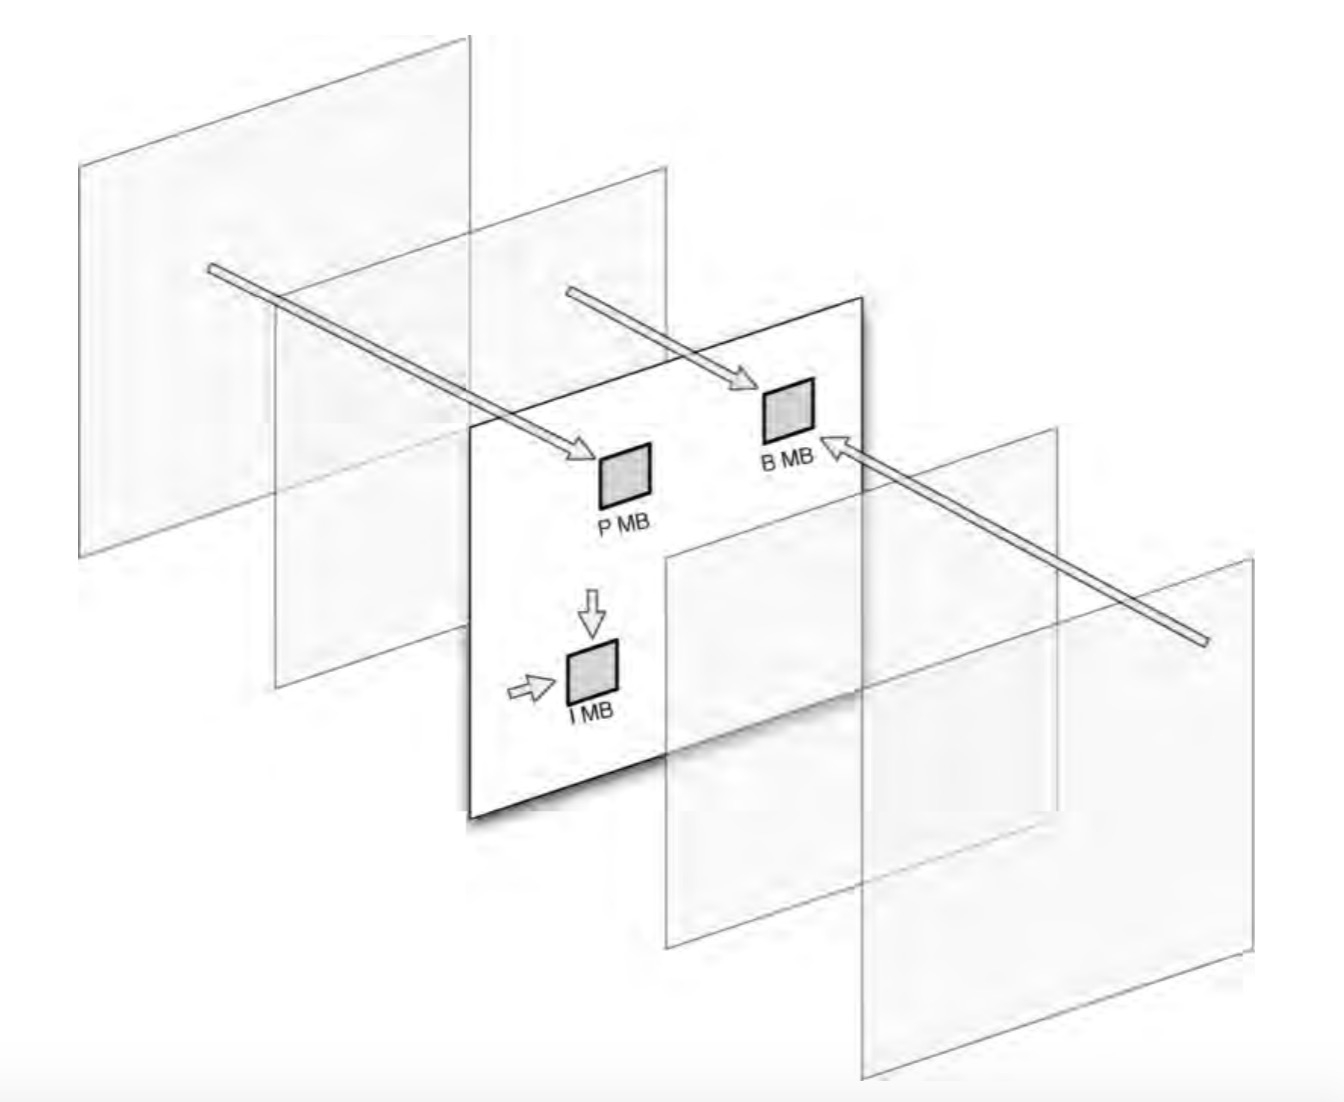
\includegraphics[height=5cm]{marcoblock.jpg}
   \end{tabular}
   \end{center}
   \caption[example] 
%>>>> use \label inside caption to get Fig. number with \ref{}
   { \label{fig:example} 
Marcoblock}
   \end{figure}     % 在reference中引用
   
\subsubsection{ Inter-Prediction }

Inter prediction is the process of predicting
a block of luma and chroma samples from a picture that has
previously been coded and transmitted, a reference picture. It
takes advantage of the fact that the content of a new frame in
the video often has high correlation to the data in the
previous frames.

Reference pictures

Macroblock partitions

Motion vector prediction








\end{document}